%%%%%%%%%%%%%%%%%%%%%%%%%%%%%%%%%%%%%
%                                   %
% Compile with XeLaTeX and biber    %
%                                   %
% Questions or comments:            %
%                                   %
% joshua dot mcneill at uga dot edu %
%                                   %
%%%%%%%%%%%%%%%%%%%%%%%%%%%%%%%%%%%%%

\documentclass{beamer}
  % Read in standard preamble (cosmetic stuff)
  %%%%%%%%%%%%%%%%%%%%%%%%%%%%%%%%%%%%%%%%%%%%%%%%%%%%%%%%%%%%%%%%
% This is a standard preamble used in for all slide documents. %
% It basically contains cosmetic settings.                     %
%                                                              %
% Joshua McNeill                                               %
% joshua dot mcneill at uga dot edu                            %
%%%%%%%%%%%%%%%%%%%%%%%%%%%%%%%%%%%%%%%%%%%%%%%%%%%%%%%%%%%%%%%%

% Beamer settings
% \usetheme{Berkeley}
\usetheme{CambridgeUS}
% \usecolortheme{dove}
% \usecolortheme{rose}
\usecolortheme{seagull}
\usefonttheme{professionalfonts}
\usefonttheme{serif}
\setbeamertemplate{bibliography item}{}

% Packages and settings
\usepackage{fontspec}
  \setmainfont{Charis SIL}
\usepackage{hyperref}
  \hypersetup{colorlinks=true,
              allcolors=blue}
\usepackage{graphicx}
  \graphicspath{{../../figures/}}
\usepackage[normalem]{ulem}
\usepackage{enumerate}

% Document information
\author{M. McNeill}
\title[FREN2001]{Français 2001}
\institute{\url{joshua.mcneill@uga.edu}}
\date{}

%% Custom commands
% Lexical items
\newcommand{\lexi}[1]{\textit{#1}}
% Gloss
\newcommand{\gloss}[1]{`#1'}
\newcommand{\tinygloss}[1]{{\tiny`#1'}}
% Orthographic representations
\newcommand{\orth}[1]{$\langle$#1$\rangle$}
% Utterances (pragmatics)
\newcommand{\uttr}[1]{`#1'}
% Sentences (pragmatics)
\newcommand{\sent}[1]{\textit{#1}}
% Base dir for definitions
\newcommand{\defs}{../definitions}


  % Packages and settings

  % Document information
  \subtitle[Révision, subjonctif]{Une révision du subjonctif}

\begin{document}
  % Read in the standard intro slides (title page and table of contents)
  \begin{frame}
    \titlepage
    \tiny{Office: % Basically a variable for office hours location
Gilbert 121\\
          Office hours: % Basically a variable for office hours
 lundi, mercredi, vendredi 10:10--11:10
}
  \end{frame}

  \begin{frame}{Qu'est-ce qu'il faut faire?}
    \small
    Avec un/e partenaire, discutez de ce qu'il faut faire pour le cours de français avant l'examen final.
    Dis au moins trois phrase, et \alert{utilise des expressions comme celles ci-dessous} au début des phrases.
    Indique si tu es d'accord avec ton/ta partenaire en ce qui concerne chaque phrase.
    \begin{columns}[t]
      \column{0.55\textwidth}
        \begin{description}
          \item[] \textbf{Modèle:}
          \item[E1:] Il est utile qu'on finisse les exercices MFL.
          \item[E2:] Je ne suis pas d'accord avec ça. Ils ne sont pas utiles.
          \item[OU] Oui, je suis d'accord avec ça. Les exercices m'aident beaucoup!
        \end{description}
      \column{0.45\textwidth}
        \begin{itemize}
          \item[] Des exemples d'expressions:
          \item Il faut que ...
          \item Il est important que ...
          \item Il est vrai que ...
          \item Je veux que ...
          \item Je préfère que ...
          \item Le prof exige que ...
          \item Il vaut mieux que ...
        \end{itemize}
    \end{columns}
  \end{frame}

  \begin{frame}{Les éco-gestes}
    Regardons les diapos \gloss{slides} que nous avons créées pendant la dernière classe.
  \end{frame}

  \begin{frame}{La bataille navale}
    \scriptsize
    \begin{columns}
      \column{0.6\textwidth}
        Jouons à la bataille navale avec un/e partenaire.
        Voici les règles:
        \begin{itemize}
          \item Tu auras 5 bateaux qui prennent les nombres de cases \gloss{squares} suivants:
          \begin{itemize}
            \scriptsize
            \item 2 cases x1
            \item 3 cases x2
            \item 4 cases x1
            \item 5 cases x1
          \end{itemize}
          \item Mets tes bateaux où que \gloss{wherever} tu veux sur le plateau.
          \item Ton/ta partenaire va deviner une case où se trouvent tes bateaux en construisant une phrase d'un mot de la colonne et un mot de la ligne.
          \begin{itemize}
            \scriptsize
            \item Par ex., Tu + parler = Tu parles
          \end{itemize}
          \item Si c'est une case où tu a un bateau, marque la case.
          \item Si toutes les cases d'un bateau sont choisies, le bateau est coulé \gloss{sunk}.
          \end{itemize}
      \column{0.4\textwidth}
        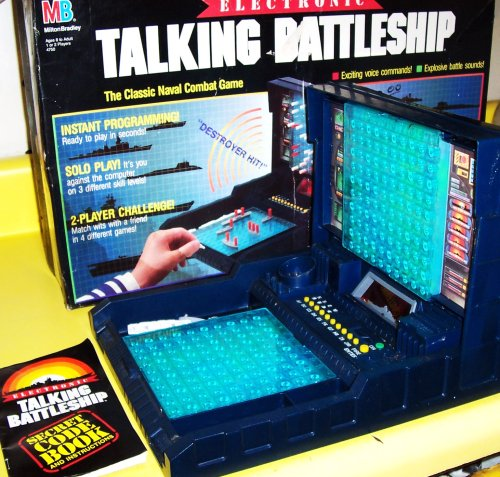
\includegraphics[scale=0.25]{battleship.jpg}
    \end{columns}
  \end{frame}

  \begin{frame}{Le subjonctif ou non, encore}
    \begin{enumerate}
      \item Il est nécessaire que tu te \underline{\uncover<2->{soignes}} (soigner).
      \item<3->[$\to$] le subjonctif
      \item Mon père veux qu'il \underline{\uncover<4->{a}} (avoir) plus de temps.
      \item<5->[$\to$] l'indicatif
      \item C'est étonnant que vous \underline{\uncover<6->{aimiez}} (aimer) tant le subjonctif!
      \item<7->[$\to$] le subjonctif
      \item Nous doutons qu'elles \underline{\uncover<8->{sautent}} (sauter) des repas.
      \item<9->[$\to$] le subjonctif
      \item Il pense que je \underline{\uncover<10->{suis}} (suivre) des régimes trop strictes, mais ce n'est pas vrai!
      \item<11->[$\to$] l'indicatif
    \end{enumerate}
  \end{frame}

  \begin{frame}{}
    \begin{center}
      \Large Questions?
    \end{center}
  \end{frame}
\end{document}
